\section{M�leopstillinger}
P� hardware-siden har vi benyttet en b�rbar Mac tilkoblet et Alesis IO|14 lydkort. Vi har foretaget m�lingerne ved hj�lp af softwaren FuzzMeasure 2.

Ved hj�lp af FuzzMeasure har vi sendt et sinus-sweep (1000 ms varighed, g�ende fra 100 Hz til 20000 Hz) igennem NXT-h�jttaleren og optaget det igen. FuzzMeasure beregner impulssvaret ved at affolde sinus-sweepet fra det optagede signal. Vi har optaget signalet ved 48000 kHz, s�ledes at vi b�de har taget Nyquist samt high-cut filteret p� lydkortets A/D-converter i betragtning. 

Til vores m�linger har vi benyttet en Behringer ECM8000 m�lemikrofon,
som har en nogelunde line�r frekvensgang indenfor det frekvensomr�de
vi er interresserede i at unders�ge, dvs. 100Hz til 20kHz. Mikrofonens
frekvens karakteristik kan ses p� figur \ref{ecm8000}.

\begin{figure}[h!]
\begin{center}
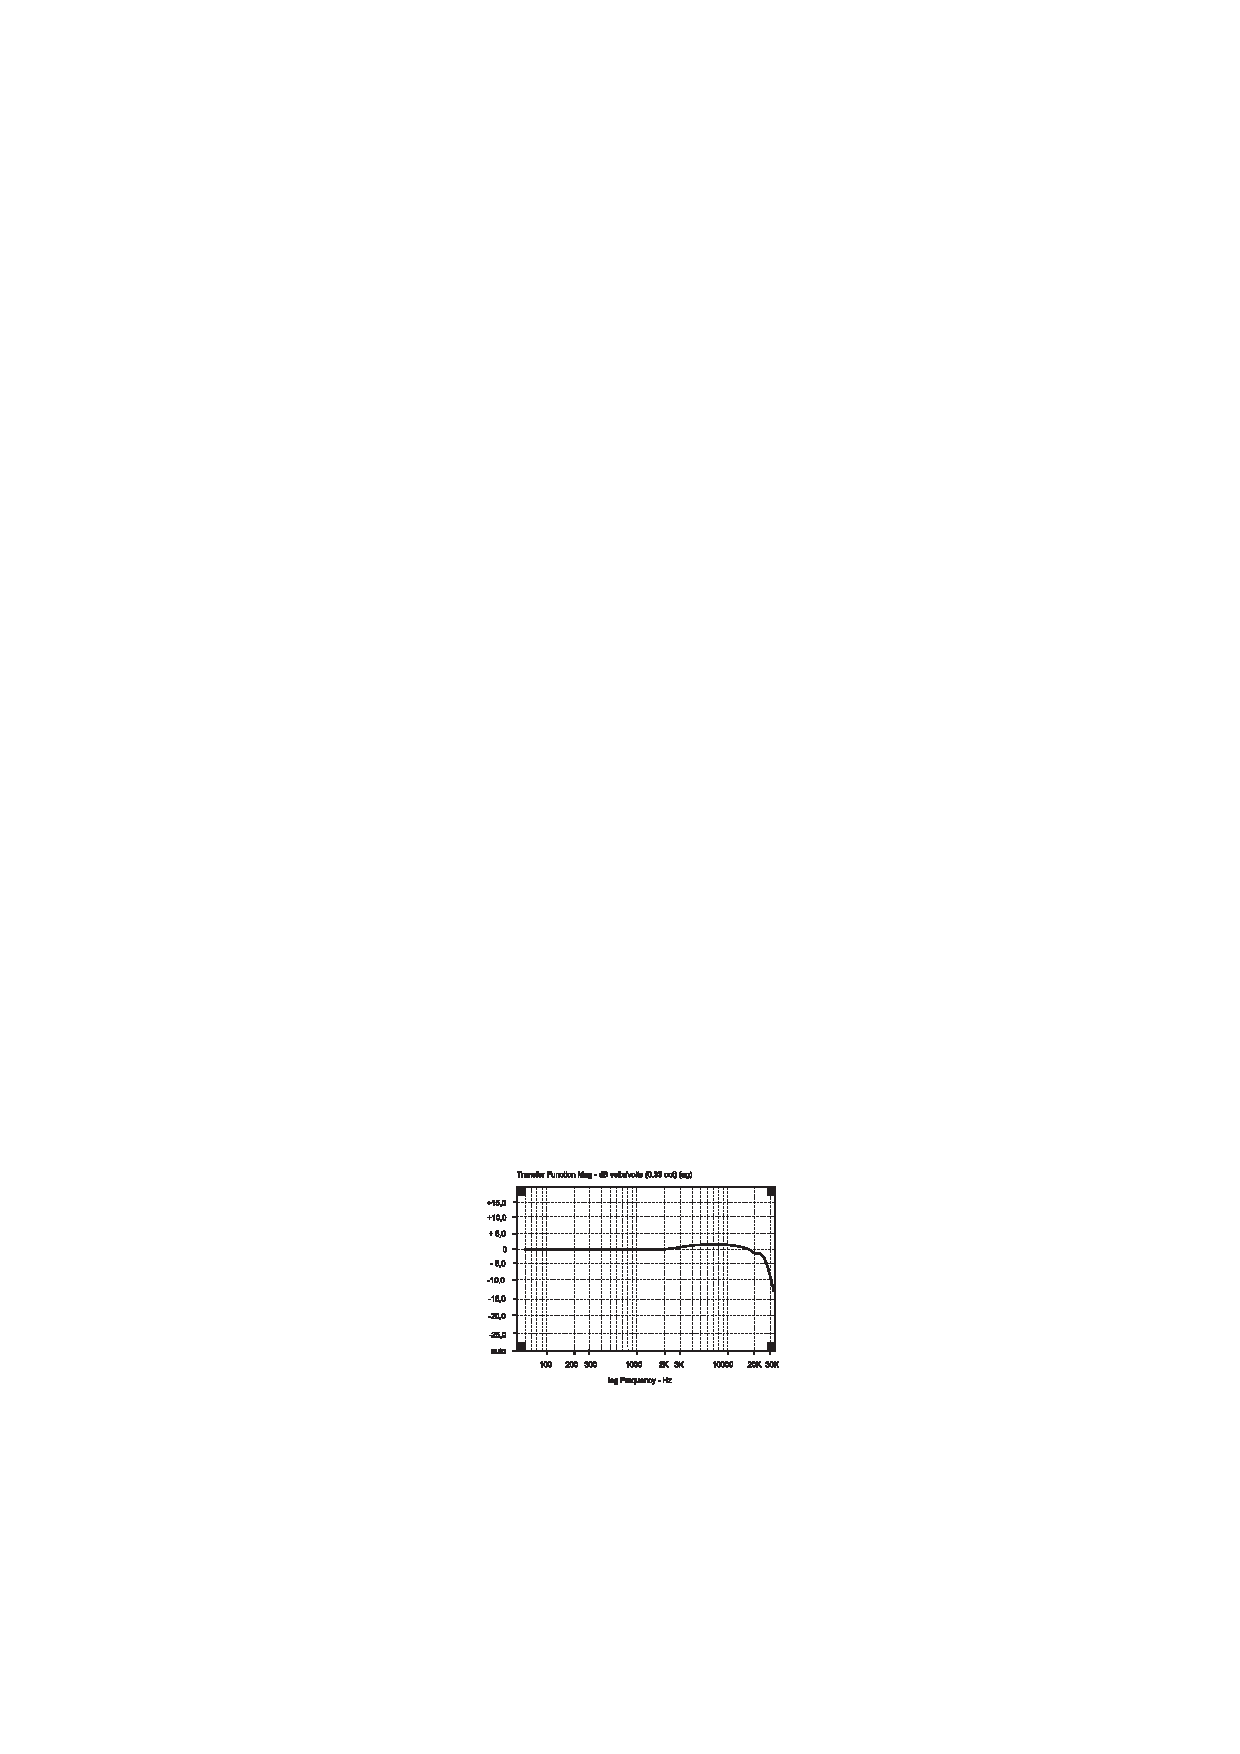
\includegraphics[width=12cm]{ecm8000_freqres.pdf}
\end{center}
\caption{Frekvensgangen p� Behringer ECM8000 mikrofonen}
\label{ecm8000}
\end{figure}

Vi har m�lt i 10 graders intervaller op til 40 grader fra on axis og i alle retninger. I alt 81 m�linger.\\
Det giver anledning til det grid over m�lingerne, som kan ses p� figur \ref{angles}.
\begin{figure}[h!]
\begin{center}
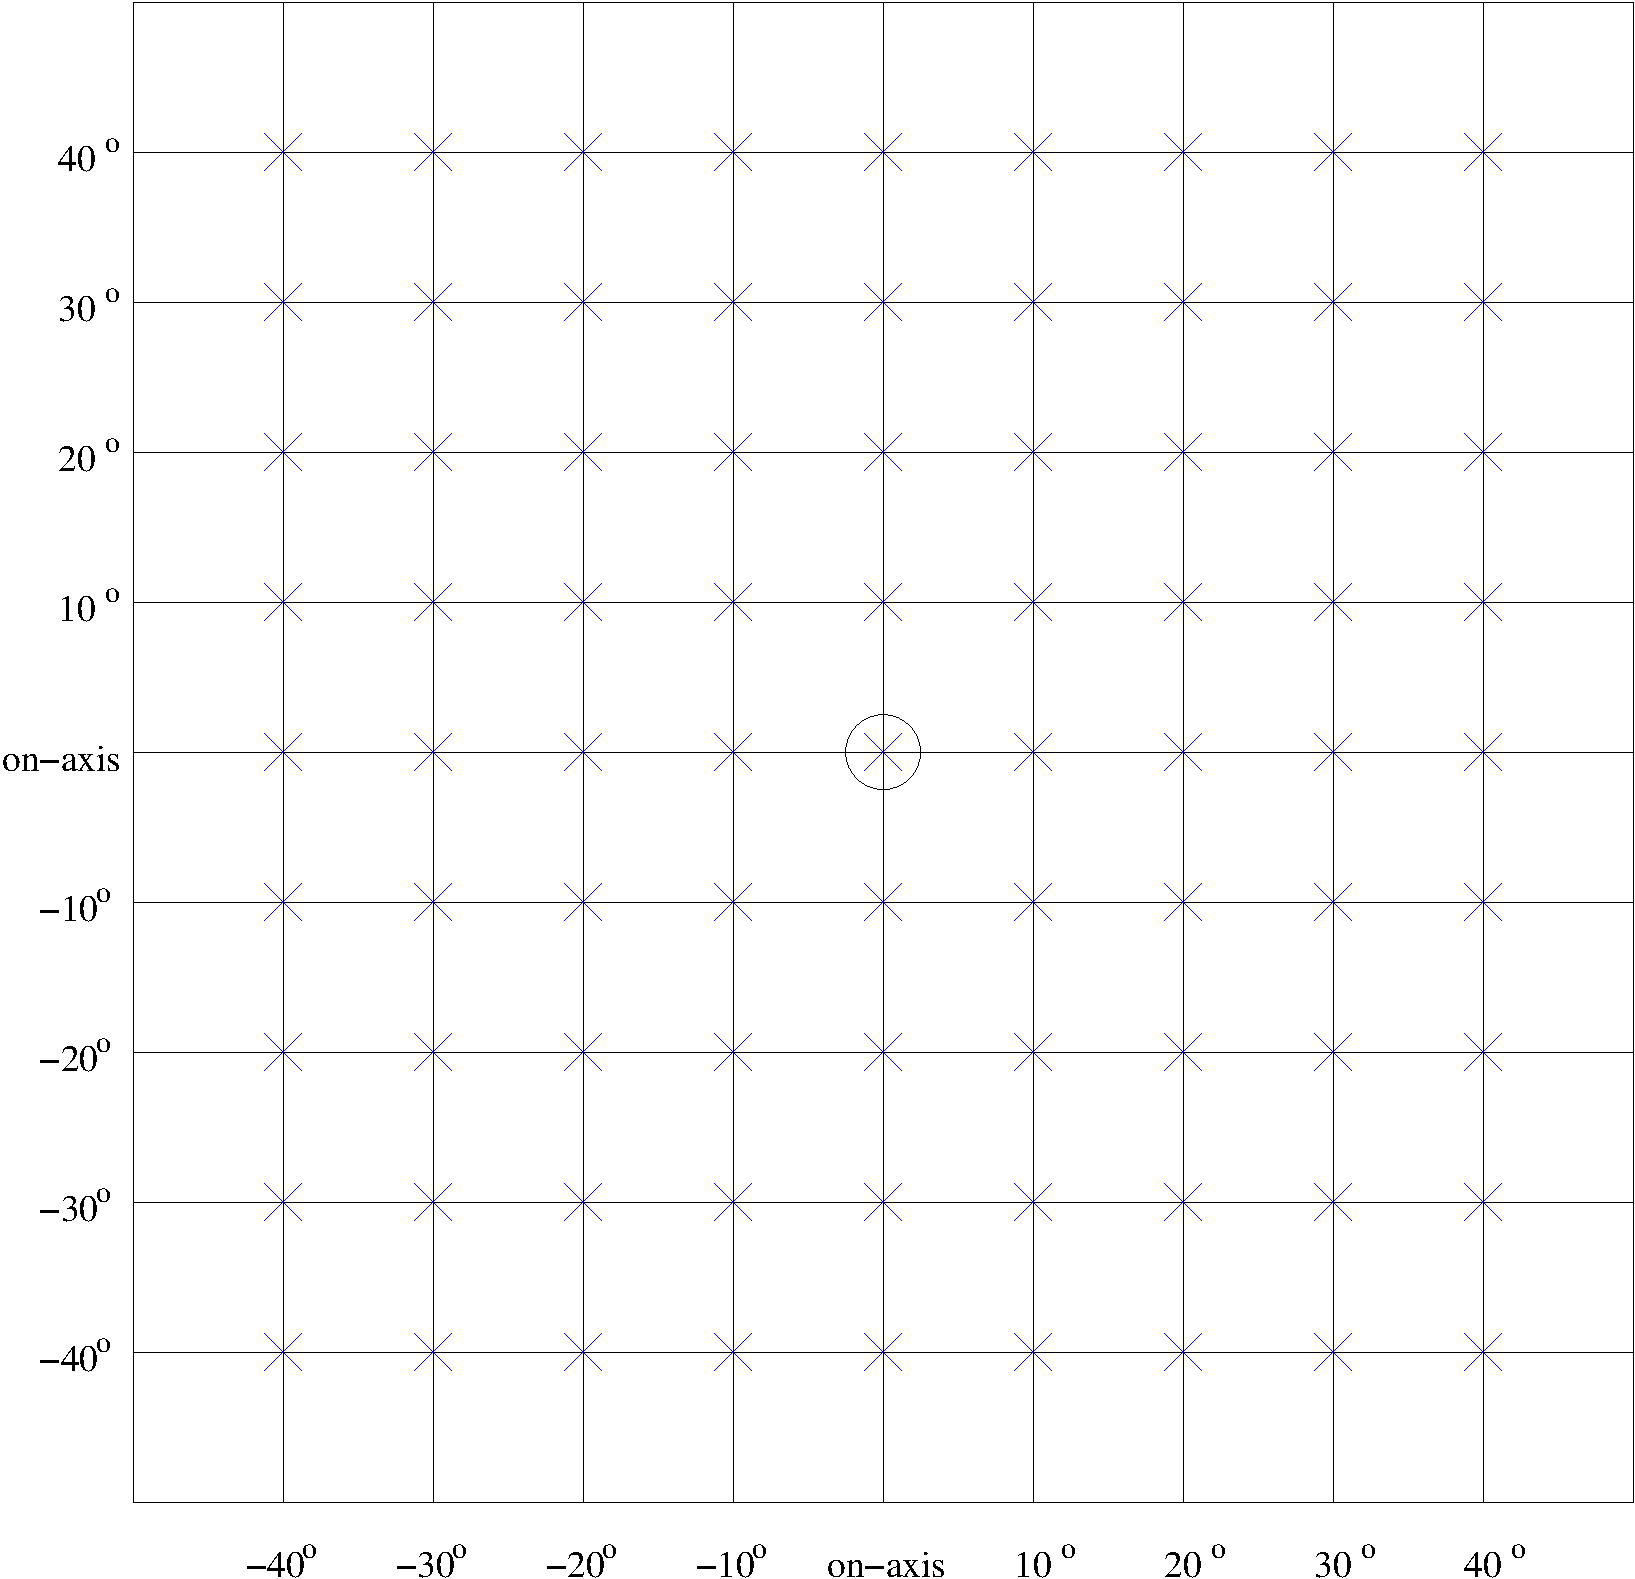
\includegraphics[width=8cm]{angles.pdf}
\end{center}
\caption{Illustration af m�lepunkterne.}
\label{anlges}
\end{figure}

Vores closerange m�linger er alle lavet ved 12 cm afstand, hhv. med og uden kabinet.

Desuden har vi foretaget m�linger p� 2 m. afstand i en vinkel p�
ca. 45 grader oppe fra. Der er her lavet m�linger hvor h�jtaleren
peger hen imod lytteren, og v�k fra lytteren, for at afspejle hvad man
kan kalde almindeligt brug.

Alle m�lingerne er foretaget i et lydd�dt rum (se figur \ref{room}), med en udefra d�mpning
p� -60dB. Rummet er approksimativt $60m^3$ med en nedre begr�nsende
frekvens p� 100Hz, svarende til starten p� vores sweep (100Hz -
20kHz).

\begin{figure}[h!]
\begin{center}
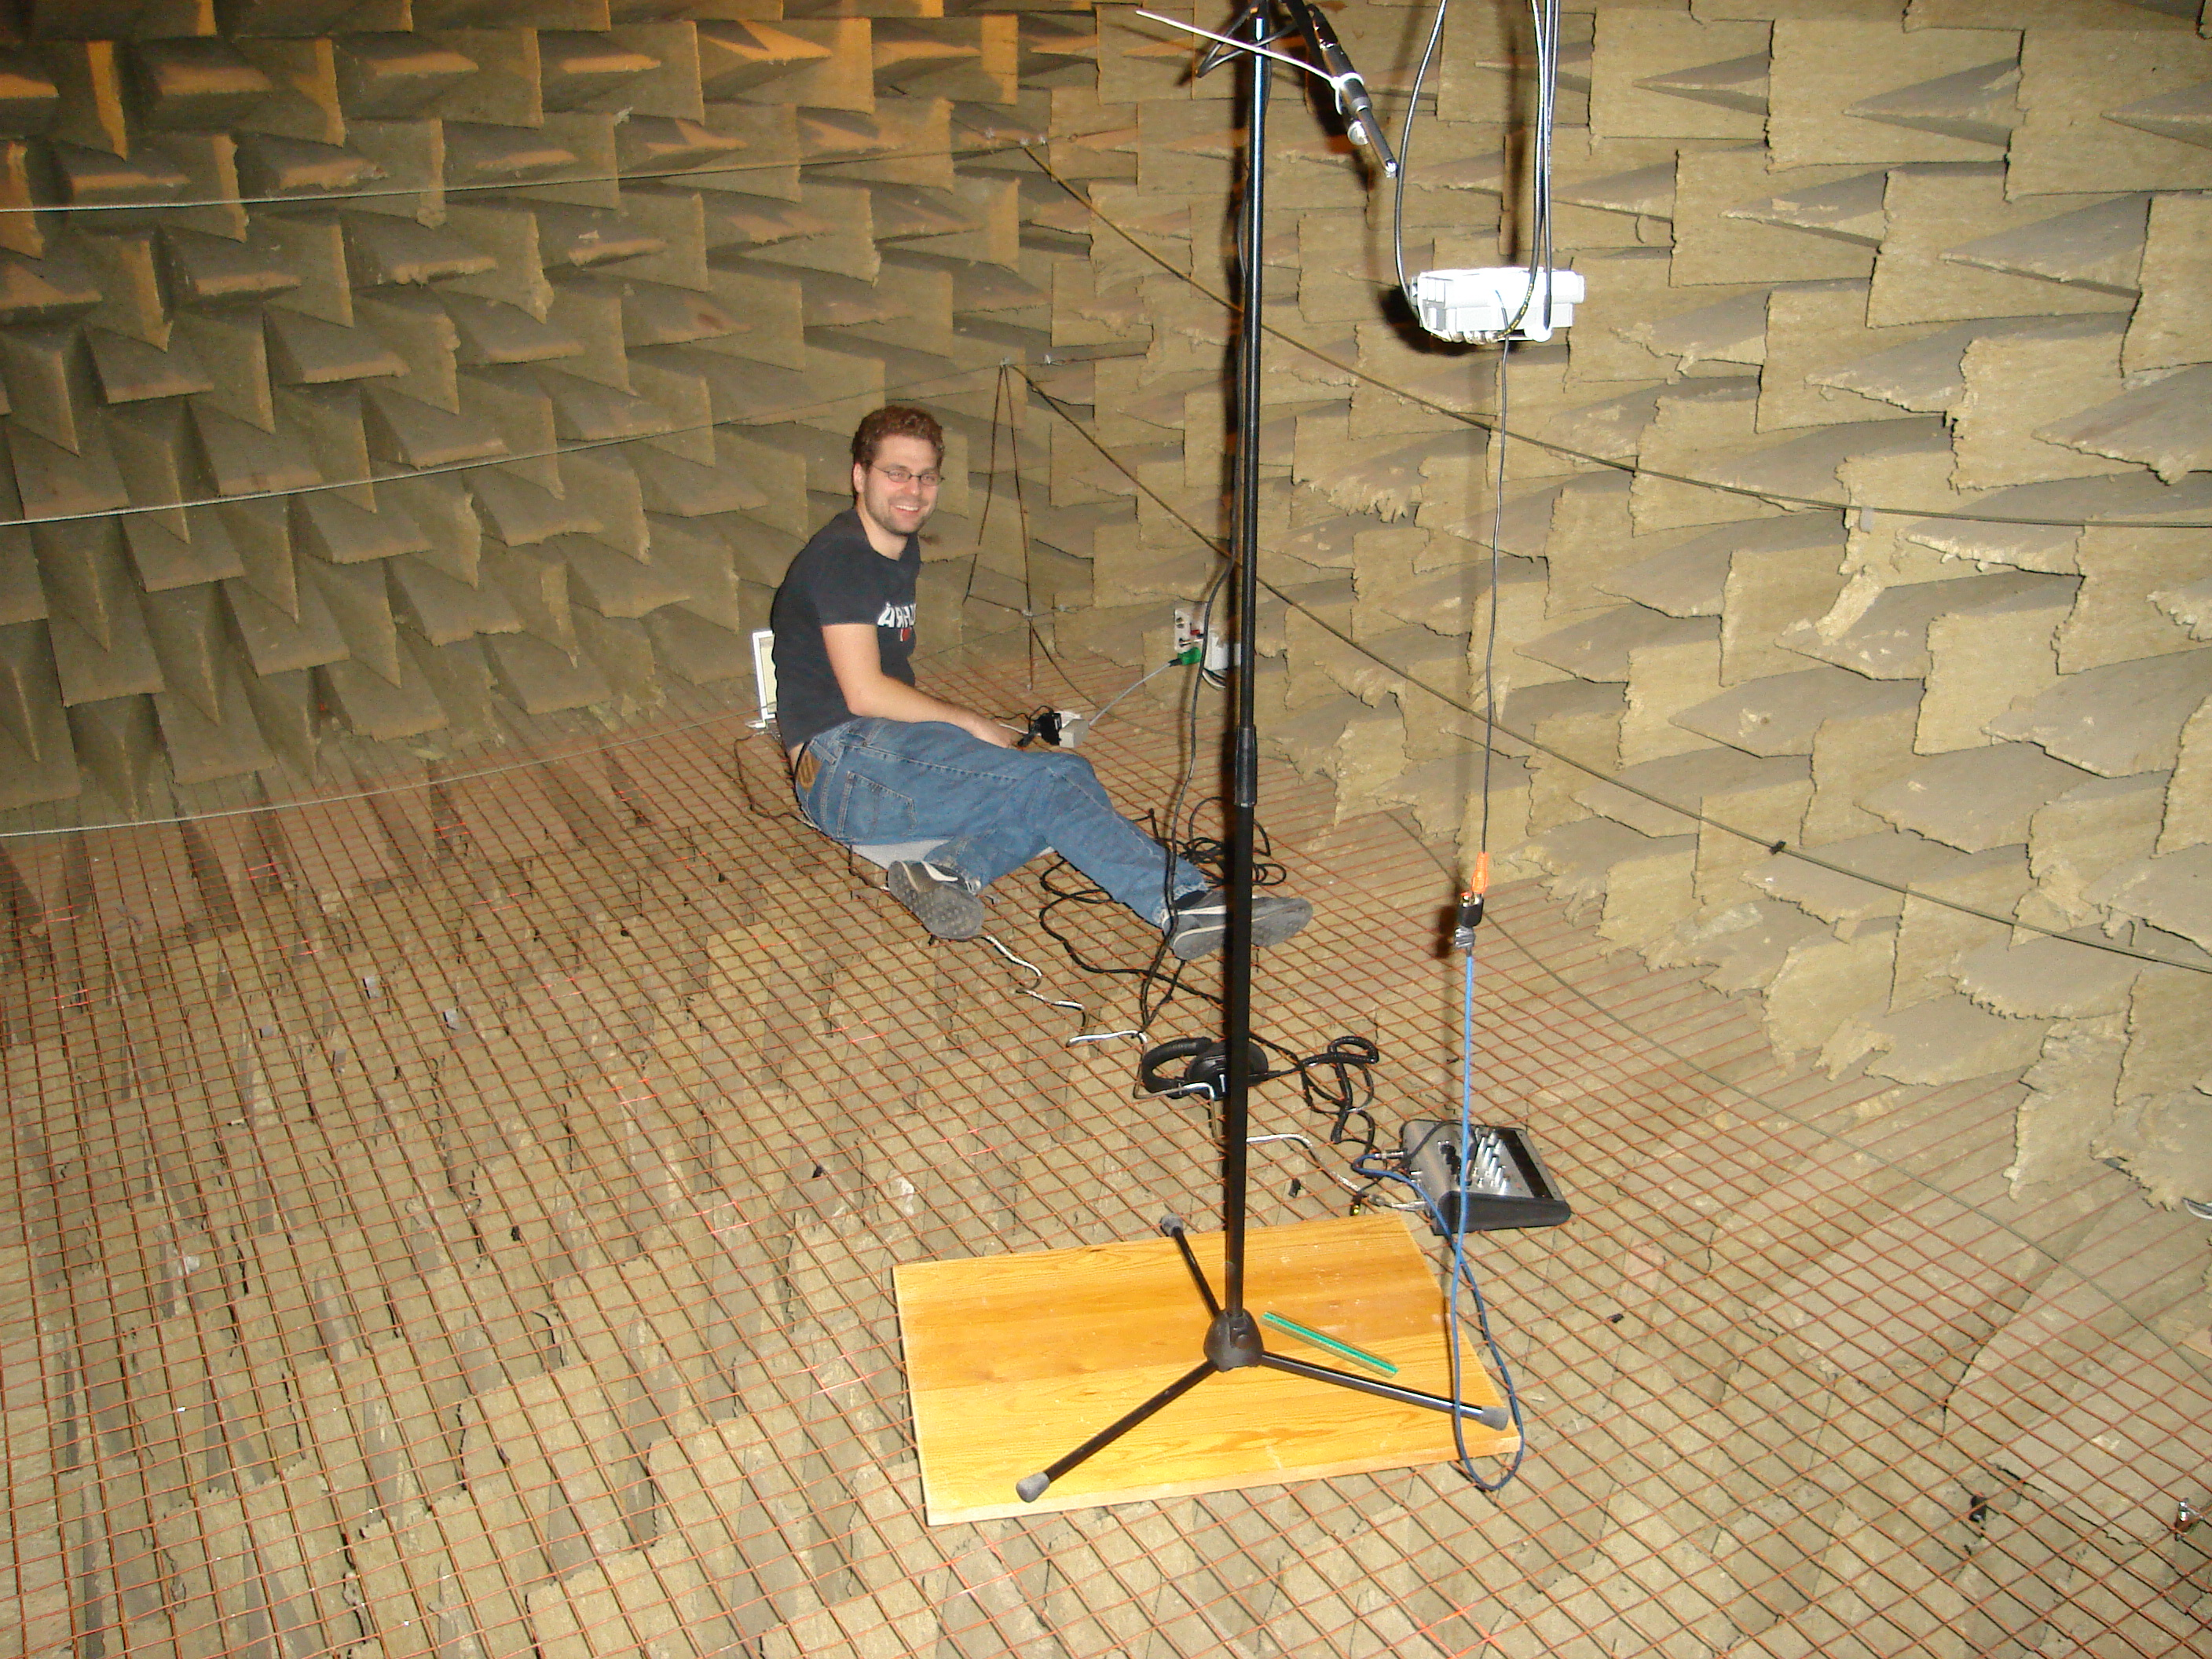
\includegraphics[width=12cm]{room.jpg}
\end{center}
\caption{M�linger blev foretaget i et lydd�dt rum.}
\label{room}
\end{figure}
